\chapter{Theoretical Foundations}\label{chap:theoretical_foundations}
This chapter delves into the mathematical and theoretical underpinnings essential for understanding the development and application of large language models (LLMs). The discussion begins with an exploration of linear algebra, which forms the cornerstone of deep learning and is instrumental in defining the operations and transformations within neural networks. It further elucidates how vectors, matrices, and tensors serve as fundamental building blocks in representing data and parameters in neural networks. 

Subsequently, the chapter examines the role of matrix operations, emphasizing the importance of matrix multiplication in transforming data across layers of a neural network. It also covers Singular Value Decomposition (SVD), a powerful technique for decomposing matrices, which is crucial for various machine learning tasks such as data compression and noise reduction.

The concept of low-rank approximation is introduced, highlighting its significance in reducing computational complexity and storage requirements, particularly in the context of deep learning where large matrices are prevalent. This section provides detailed insights into how low-rank approximation achieves efficiency gains without significantly compromising the quality of neural network outputs.

Additionally, the chapter discusses neural networks, focusing on their architecture, learning processes, optimization, and regularization techniques. It explains how neural networks are designed to capture and transmit abstract features through layers of interconnected nodes, and how they are trained to perform specific tasks through optimization algorithms and regularization methods.

Lastly, the chapter provides an understanding of cosine similarity, a metric used to measure the similarity between vectors, and its relevance in text analysis and NLP applications. The chapter culminates with an overview of large language models, detailing their architecture based on the Transformer model, the attention mechanisms that enable them to capture context, and the training and fine-tuning processes that enhance their performance on various NLP tasks.

\section{Linear Algebra in Deep Learning}
Linear algebra forms the cornerstone of deep learning, providing the necessary mathematical framework to model and understand complex relationships within data. It is instrumental in defining the operations and transformations that occur within deep neural networks, including those underlying LLMs.

\subsection{Vectors, Matrices, and Tensors}
Vectors and matrices are fundamental to representing data and parameters in neural networks. A vector $\mathbf{v} \in \mathbb{R}^n$ can represent a point in $n$-dimensional space or a single data instance with $n$ features. Matrices $A \in \mathbb{R}^{m \times n}$ facilitate linear transformations from $\mathbb{R}^n$ to $\mathbb{R}^m$, and tensors generalize these concepts to higher dimensions, accommodating the multi-dimensional data structures processed by neural networks.

A typical case, representing a basic neural network operation, can be expressed as:
\begin{equation}
    \mathbf{y} = A\mathbf{x} + \mathbf{b}
    \label{eq:matrix_multiplication}
\end{equation}
where $A$ is the weight matrix, $\mathbf{x}$ is the input vector, $\mathbf{b}$ is the bias vector, and $\mathbf{y}$ is the output vector of the transformation.

\subsection{Matrix Operations}
    Matrix operations such as addition, multiplication, and transposition are essential in neural network computations. Matrix multiplication, in particular, plays a crucial role in transforming data between layers, capturing the relationships between input and output features. The dot product of two matrices $A \in \mathbb{R}^{m \times n}$ and $B \in \mathbb{R}^{n \times p}$ is defined as:
    \begin{equation}
        C = AB = \sum_{i=1}^{n} A_{ij}B_{jk}
        \label{eq:matrix_multiplication}
    \end{equation}
    where $C \in \mathbb{R}^{m \times p}$ is the resulting matrix. Matrix multiplication is a key operation in neural networks, enabling the transformation of input data through multiple layers of weights and biases.
    
    \subsubsection{Floating-Point Operations}
    Floating-point operations (FLOPs) are a measure of the computational complexity of matrix operations. The number of FLOPs required for matrix multiplication is proportional to the product of the dimensions of the matrices involved. For example, the number of FLOPs for multiplying two matrices $A \in \mathbb{R}^{m \times n}$ and $B \in \mathbb{R}^{n \times p}$ is $2mnp$ (\cite{swann2022numerisk}). Furtherly, the number of FLOPs required for a matrix-vector multiplication of matrix $A \in \mathbb{R}^{m \times n}$ and vector $\mathbf{x} \in \mathbb{R}^n$ is $2mn$ (\cite{swann2022numerisk}).

\subsection{Singular Value Decomposition}
    Singular Value Decomposition (SVD) is a powerful technique for decomposing a matrix into singular vectors and singular values, providing insight into the structure of the data. For any matrix $A \in \mathbb{R}^{m \times n}$, SVD is given by:
    \begin{equation}
        A = U\Sigma V^T
        \label{eq:svd}
    \end{equation}
    where $U$ and $V$ are orthogonal matrices containing the left and right singular vectors, respectively, and $\Sigma$ is a diagonal matrix with singular values. SVD is essential in many machine learning tasks, including noise reduction, data compression, and the analysis of neural network layers.

\subsection{Low-Rank Approximation}

    Low-rank approximation is an effective technique in linear algebra that can provide significant benefits in terms of computational efficiency and storage requirements. This method is particularly useful in the context of deep learning, where large matrices are frequently encountered, and computational resources are often a limiting factor.
    
    \subsubsection{Concept of Low-Rank Approximation}
    
    Given a matrix $A$ of dimensions $m \times n$, low-rank approximation aims to approximate $A$ by another matrix $A_k$ of lower rank $k$, where $k$ is much smaller than both $m$ and $n$. A version of this approximation leverages the Singular Value Decomposition (SVD) of $A$:
    
    \[
    A \approx A_k = U_k \Sigma_k V_k^T
    \]
    
    Here:
    \begin{itemize}
        \item $U_k$ is an $m \times k$ matrix containing the top $k$ left singular vectors.
        \item $\Sigma_k$ is a $k \times k$ diagonal matrix containing the top $k$ singular values.\footnote{While it is possible to represent $\Sigma_k$ as a $k$-element vector, choosing a $k \times k$ matrix allows for more flexibility in mathematical operations and maintains consistency in the representation of the decomposition, which can simplify implementation and theoretical analysis.}
        \item $V_k^T$ is a $k \times n$ matrix containing the top $k$ right singular vectors.
    \end{itemize}
    
    This decomposition allows $A_k$ to capture the most significant components of $A$, effectively reducing its rank while preserving its essential characteristics.
    
    \subsubsection{Reduction in Storage}\label{sec:reduction_storage}
    
    The primary benefit of low-rank approximation is the significant reduction in storage requirements. Instead of storing the original matrix $A$ with $m \times n$ elements, the low-rank approximation stores the three smaller matrices $U_k$, $\Sigma_k$, and $V_k^T$:
    
    \begin{itemize}
        \item $U_k$ with $m \times k$ elements.
        \item $\Sigma_k$ with $k \times k$ elements.
        \item $V_k^T$ with $k \times n$ elements.
    \end{itemize}
    Thus, making the total number of elements required to store these matrices:
    \begin{displaymath}
        m \times k + k \times k + k \times n = k(m + k + n)
    \end{displaymath}
    For \(k\) much smaller than \(m\) and \(n\), this results in a substantial reduction in storage.\\
    For example, consider a matrix \(A\) of size \(1000 \times 1000\). If we approximate \(A\) with rank \(k = 50\) we have:
    \begin{itemize}
        \item Original Matrix: \(1000 \times 1000 = 1000000\) elements.
        \item Low-rank approximation: \(1000 \times 50 + 50 \times 50 + 50 \times 1000 = 102500\) elements.
    \end{itemize}
    which is a substantial reduction in storage requirements.\\
    But if we choose \(k = 500\), the low-rank approximation would require 
    \begin{displaymath}
        1000 \times 500 + 500 \times 500 + 500 \times 1000 = 1250000 \text{ elements,}
    \end{displaymath} which is more than the original matrix \(A\). Thus, the choice of \(k\) is crucial in achieving storage reduction.\\
    More specifically, we want
    \begin{gather*}
        k(m+k+n) = k^2 + k(m+n) < mn \\
        \Updownarrow \\
        k^2 + k(m+n) - mn < 0 \\
        \Updownarrow \\
        k < \frac{\sqrt{4mn + (m+n)^2} - m - n}{2}
    \end{gather*}
    This inequality provides a guideline for selecting an appropriate rank \(k\) to achieve storage reduction.
    
    \subsubsection{Reduction in Computation for Matrix-Vector Multiplications}
    
    Low-rank approximation can also reduce the computational complexity of various matrix operations. In the case of a matrix-vector multiplication we have:
    
    \begin{itemize}
        \item \textbf{Original Matrix}: Multiplying $A$ (size $m \times n$) with a vector (size $n$) requires $2mn$ FLOPs.
        \item \textbf{Low-Rank Approximation}: Multiplying $A_k = U_k \Sigma_k V_k^T$ with a vector involves three steps:
        \begin{itemize}
            \item $V_k^T$ with the vector: $2kn$ FLOPs,
            \item $\Sigma_k$ multiplication: $2k^2$ FLOPs.
            \item $U_k$ multiplication: $2mk$ FLOPs.
        \end{itemize}
        \item \textbf{Total}: $2kn + 2k^2 + 2mk = 2k(k + m + n)$ FLOPs.
    \end{itemize}
    Therefore, the appropriate choice of rank \(k\) to achieve computational efficiency for matrix-vector multiplications is
    \begin{gather*}
        2kn + 2k^2 + 2mk = 2k(k + m + n) < 2mn \\
        \Updownarrow \\
        k < \frac{\sqrt{4mn + (m+n)^2} - m - n}{2}
    \end{gather*}
    
    \subsubsection{Reduction in Computation for Matrix-Matrix Multiplications}
    In the case of a matrix-matrix multiplication we have:
    
    \begin{itemize}
        \item \textbf{Original Matrix}: Multiplying $A$ (size $m \times n$) with another matrix of size $n \times p$ requires $2mnp$ FLOPs.
        \item \textbf{Low-Rank Approximation}: Multiplying $A_k = U_k \Sigma_k V_k^T$ with a matrix of size $n \times p$ involves:
        \begin{itemize}
            \item $V_k^T$ with the matrix: $2knp$ FLOPs.
            \item $\Sigma_k$ multiplication: $2k^2p$ FLOPs.
            \item $U_k$ multiplication: $2mkp$ FLOPs.
        \end{itemize}
        \item \textbf{Total}: $2knp + 2k^2p + 2mkp = 2k(k + m + n)p$ FLOPs.
    \end{itemize}
    Therefore, the appropriate choice of rank \(k\) to achieve computational efficiency for matrix-matrix multiplications is also
    \begin{displaymath}
        k < \frac{\sqrt{4mn + (m+n)^2} - m - n}{2}
    \end{displaymath}
    
    By choosing a sufficiently small $k$, the amount of FLOPs can be reduced compared to when using the full-rank matrix $A$.\\
    Thus, making low-rank approximation via SVD a powerful technique that offers significant benefits in terms of storage reduction and computational efficiency. By focusing on the most important components of a matrix, low-rank approximation makes it feasible to handle large datasets and complex computations more effectively, which is crucial in the field of deep learning and beyond.
    
\subsection{Neural Networks in Deep Learning}
   A Neural network consist of interconnected nodes or "neurons" arranged in layers, with each layer designed to perform specific transformations on its inputs to capture and transmit increasingly abstract features to subsequent layers.
    
    \subsubsection{Architecture of Neural Networks}
    The architecture of a neural network is defined by layers, each comprising a set of neurons connected by weights. These weights are adjusted during the training process to minimize the difference between the actual output of the network and the desired output. A typical feedforward neural network can be mathematically represented as:
    \begin{equation}
        \mathbf{h}^{(l)} = f(W^{(l)}\mathbf{h}^{(l-1)} + \mathbf{b}^{(l)})
    \end{equation}
    where $W^{(l)}$ and $\mathbf{b}^{(l)}$ are the weight matrix and bias vector for the $l$-th layer, $\mathbf{h}^{(l-1)}$ is the output from the previous layer, and $f$ is a non-linear activation function such as ReLU or sigmoid.
    
    \subsubsection{Learning Process}
    The learning process in neural networks involves adjusting weights and biases to reduce a loss function, commonly through backpropagation. This method efficiently computes gradients using calculus' chain rule:
    \begin{equation}
        W^{(l)} \leftarrow W^{(l)} - \eta \frac{\partial \mathcal{L}}{\partial W^{(l)}}
    \end{equation}
    where $\eta$ is the learning rate and $\mathcal{L}$ is the loss function.
    
    \subsubsection{Optimization and Regularization}
    Optimization algorithms like Stochastic Gradient Descent (SGD), Adam, and RMSprop are crucial for weight updates. Regularization techniques such as dropout and weight decay help prevent overfitting, ensuring the network generalizes well to new data.
    
\subsection{Cosine Similarity}
The cosine similarity between two vectors $\mathbf{a}$ and $\mathbf{b}$ is defined as:
\[
S_c(\mathbf{a}, \mathbf{b}) = \frac{\mathbf{a} \cdot \mathbf{b}}{\|\mathbf{a}\| \|\mathbf{b}\|}
\]
where $\mathbf{a} \cdot \mathbf{b}$ is the dot product of $\mathbf{a}$ and $\mathbf{b}$, and $\|\mathbf{a}\|$ and $\|\mathbf{b}\|$ are the magnitudes (or norms) of vectors $\mathbf{a}$ and $\mathbf{b}$, respectively.

Cosine similarity is a metric used to measure the cosine of the angle between two non-zero vectors in an inner product space. It is particularly useful in the context of text analysis and NLP, where it quantifies the similarity between two vectors of an inner product space that represents the words or documents.

By applying cosine similarity, models can effectively capture the similarity in high-dimensional data, making it a valuable tool in various machine learning and deep learning applications.


\section{Understanding LLMs}
    LLMs such as GPT (Generative Pre-trained Transformer) and BERT (Bidirectional Encoder Representations from Transformers) have revolutionized the field of NLP by leveraging deep neural networks to understand and generate human-like text unlocking a whole host of new applications.


    \subsection{The Concept of LLMs?}
        LLMs are deep neural networks trained on vast amounts of text data. They learn to predict the next word in a sentence, understand context, generate text, and perform various NLP tasks with minimal task-specific adjustments. The strength of LLMs lies in their ability to capture intricate patterns in language through extensive pre-training.
       
       
        \subsection{Architecture of LLMs}
        The architecture of most LLMs is based on the Transformer model, introduced by \cite{vaswani2023attention}, which relies on self-attention mechanisms to weigh the significance of different words in a sentence. The Transformer architecture is composed of two main components: an encoder and a decoder. The encoder takes the input text and produces a sequence of hidden states, which represent the meaning of the text. The decoder then takes the encoder's hidden states and generates the output text, one word at a time.
            \begin{figure}[h!]
                \centering
                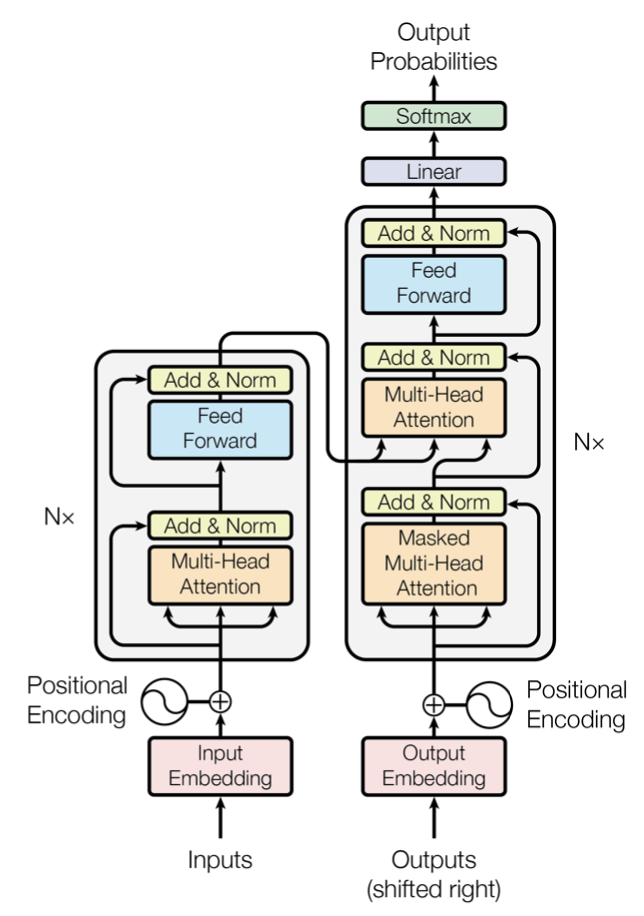
\includegraphics[width=0.5\textwidth]{figs/transform_model.png}
                \caption{Transformer model architecture - Taken from “Attention Is All You Need“ by \cite{vaswani2023attention}.}
            \end{figure}

            At a high level, the goal of the Transformer is to take an input text and predict the next word in the sequence. The input text is broken into tokens, which are typically words or parts of words. Each token is then represented as a high-dimensional vector, known as its embedding. Initially, these embeddings encode only the individual meaning of the tokens without any contextual information.

            \subsubsection{Encoder}
            The encoder consists of a stack of \(N\) identical layers, each containing two sub-layers: a multi-head self-attention mechanism and a feed-forward neural network. Furtherly, a residual connection is employed around each of the two sub-layers, followed by layer normalization. So the output of each sub-layer is \(\text{LayerNorm}(x + \text{SubLayer} (x))\), where \(\text{SubLayer}(x)\) represents the function implemented by the sub-layer.
            
            The self-attention mechanism allows the model to weigh the importance of different words in the input sequence when generating the output. The feed-forward neural network processes the output of the self-attention mechanism to produce the final hidden states of the encoder. A key feature of the encoder is that it processes all words in the input sequence in parallel, which contributes to the efficiency of the Transformer model. The output of the encoder is a sequence of vectors, each representing an input word in a high-dimensional space.

            \subsubsection{Decoder}
                The decoder, on the other hand, also consists of a stack of \(N\) identical layers, but with an additional third sublayer in each decoder layer, which performs multi-head attention over the encoder's output. This allows the decoder to focus on different parts of the encoder's output for each word in the output sequence. In the first sublayer of the decoder, self-attention is used, but with a constraint (masking) to prevent positions from attending to subsequent positions. This ensures that the predictions for position \(i\) can depend only on the known outputs at positions less than \(i\). The purpose of the decoder is to generate an output sequence one word at a time, using the encoder's output and what it has produced so far as inputs.

            \subsubsection{Attention}
                The attention mechanism is a cornerstone of the Transformer model. Its primary function is to dynamically adjust the importance of each word in the input sequence based on its context, thereby refining the embeddings of these words to capture richer meanings.

                The attention mechanism allows each token to attend to every other token in the sequence, effectively allowing the model to focus on the most relevant parts of the input when making predictions. This process is mathematically described as follows:

                \begin{equation}
                    \text{Attention}(Q, K, V) = \text{softmax}\left(\frac{QK^T}{\sqrt{d_k}}\right)V
                    \label{eq:attention}
                \end{equation}

                Here, \(Q\), \(K\), and \(V\) are the query, key, and value matrices, respectively. These matrices are derived from the input embeddings by multiplying them with learned weight matrices. The dimension \(d_k\) is the size of the key vectors and serves to scale the dot products to prevent them from growing too large.

                To understand how this works, consider a simple example: The phrases
                \begin{itemize}
                    \item "After dinner, they enjoyed a sticky \emph{date} pudding."
                    \item "She circled the \emph{date} of the concert on her calender."
                    \item "They went on their first \emph{date} to the zoo."
                \end{itemize}
                The word "date" has different meanings in each phrase, but its initial embedding would be the same. The attention mechanism helps to refine the meaning of "date" based on its context by allowing the embeddings of surrounding words to influence it.

                \textbf{Steps of the Attention Mechanism}:
                \begin{enumerate}
                    \item \textbf{Compute Query, Key, and Value Vectors:} For each embedded token \(\overrightarrow{E_i}\), we compute query (\(\overrightarrow{Q_i}\)), key (\(\overrightarrow{K_i}\)), and value (\(\overrightarrow{V_i}\)) vectors by multiplying the token's embedding with learned matrices \(W^Q\), \(W^K\), and \(W^V\):
                    \[
                    \overrightarrow{Q_i} = W^Q\overrightarrow{E_i}, \quad \overrightarrow{K_i} = W^K\overrightarrow{E_i}, \quad \overrightarrow{V_i} = W^V\overrightarrow{E_i}
                    \]

                    \item \textbf{Compute Attention Scores:} Calculate the dot products of the query vectors with all key vectors to measure how much focus each word should have on every other word, and divide by the square root of the key dimension for numerical stability:
                    \[
                    \text{Scores} = \frac{QK^T}{\sqrt{d_k}}
                    \]

                    \item \textbf{Apply Softmax Activation:} Normalize these scores using the softmax function to obtain attention weights:
                    \[
                    \text{Attention Weights} = \text{softmax}\left(\frac{QK^T}{\sqrt{d_k}}\right)
                    \]

                    \item \textbf{Compute Weighted Sum of Values:} Multiply the attention weights by the value vectors to get the final output for each token:
                    \[
                    \text{Output} = \text{softmax}\left(\frac{QK^T}{\sqrt{d_k}}\right) V
                    \]
                \end{enumerate}
                which finally leaves us with Eq. \ref{eq:attention}.
                \begin{figure}[H]
                    \centering
                    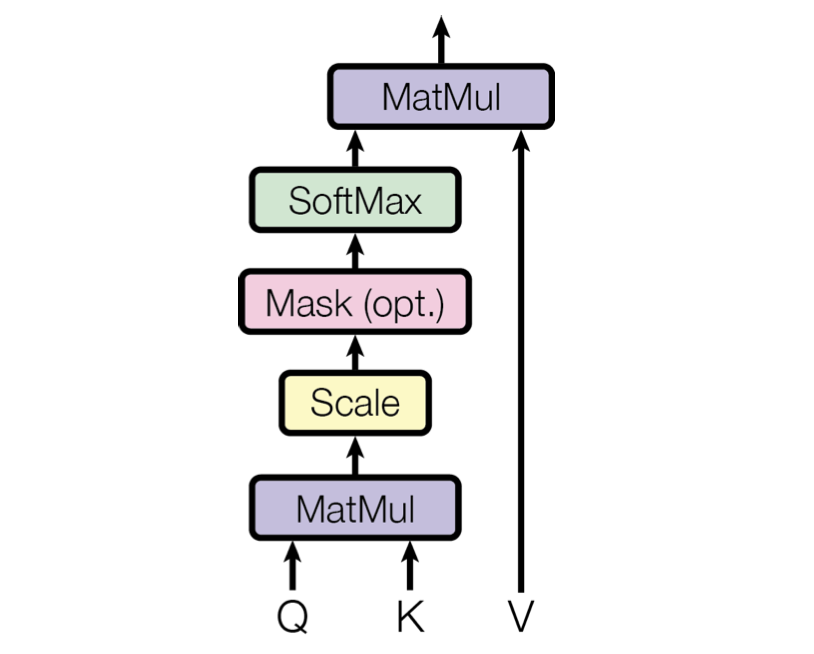
\includegraphics[width=0.6\textwidth]{figs/Scaled_dot_product.png}
                    \caption{Illustration of the Attention Mechanism - Taken from "Attention Is All You Need" by \cite{vaswani2023attention}.}
                    \label{fig:attention_mechanism}
                \end{figure}

                This mechanism allows the model to dynamically adjust which parts of the input sequence to focus on, thereby capturing the contextual meaning of each word. This whole process is described as a single 'head' of attention, and multiple heads can be used in parallel to capture different aspects of the input sequence, as elaborated in section \ref{Multi-head Attention}.

            \subsubsection{Multi-head Attention}\label{Multi-head Attention}
                Multi-head attention extends the single-head attention mechanism by allowing the model to attend to different parts of the input sequence simultaneously, capturing a variety of relationships and patterns. Instead of performing a single attention function, multi-head attention projects the queries, keys, and values into multiple subspaces and performs the attention function in each subspace independently.

                This process is mathematically described as follows:

                \begin{align}
                    \text{MultiHead}(Q, K, V) &= \text{Concat}(\text{head}_1, \ldots, \text{head}_h)W^O \\
                    \textbf{where } \text{head}_i &= \text{Attention}(QW_i^Q, KW_i^K, VW_i^V)
                \end{align}

                Here the projections are the learned parameter matrices  \(W_i^Q\), \(W_i^K\), and \(W_i^V\) for the \(i\)-th head, and \(W^O\) is the output matrix.

                \textbf{Steps of Multi-head Attention}:
                \begin{enumerate}
                    \item \textbf{Linear Projections}: Project the input embeddings into \(h\) different subspaces using learned weight matrices to create multiple sets of queries, keys, and values:
                    \[
                    Q_i = QW_i^Q, \quad K_i = KW_i^K, \quad V_i = VW_i^V
                    \]

                    \item \textbf{Parallel Attention Heads}: Apply the attention mechanism to each set of projections in parallel, producing multiple attention outputs:
                    \[
                    \text{head}_i = \text{Attention}(Q_i, K_i, V_i)
                    \]

                    \item \textbf{Concatenate and Project}: Concatenate the outputs of all attention heads and project them back to the original embedding space using a final learned matrix \(W^O\):
                    \[
                    \text{MultiHead}(Q, K, V) = \text{Concat}(\text{head}_1, \ldots, \text{head}_h)W^O
                    \]
                \end{enumerate}
                Multi-head attention allows the model to capture different aspects of the input sequence in parallel, which enhances its ability to understand complex patterns and dependencies in the data.
                \begin{figure}[H]
                    \centering
                    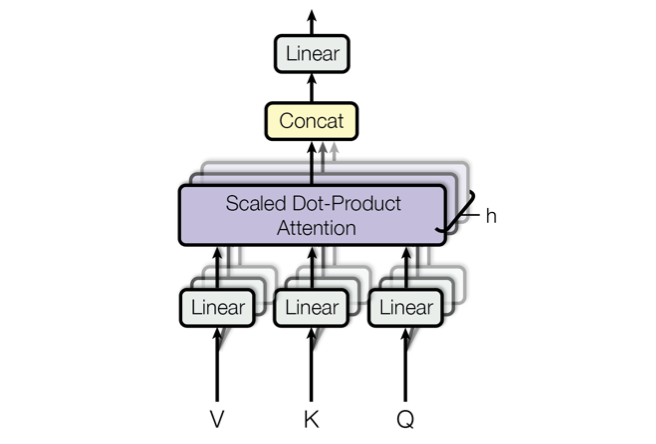
\includegraphics[width=0.6\textwidth]{figs/Multi_head_attention.png}
                    \caption{Illustration of Multi-head Attention - Taken from "Attention Is All You Need" by \cite{vaswani2023attention}.}
                    \label{fig:multi_head_attention}
                \end{figure}
                In summary, the attention and multi-head attention mechanisms enable the Transformer model to focus on relevant parts of the input sequence dynamically, improving its ability to capture context and generate accurate predictions. These mechanisms are crucial to the model's success in various NLP tasks.
                                        
                
                \subsubsection{Why Transformers?}
                The Transformer model has several advantages over traditional Recurrent Neural Networks (RNNs) and Long Short-Term Memory (LSTMs), including the ability to capture long-range dependencies, parallelize computation, and scale to larger datasets. The self-attention mechanism allows the model to focus on relevant parts of the input sequence, enabling it to learn complex patterns in the data. The multi-head attention mechanism further enhances the model's ability to capture different aspects of the input sequence in parallel, improving its performance on a wide range of NLP tasks such as translation, summarization, and image captioning. This is why Transformers have become the architecture of choice for many state-of-the-art NLP models, including GPT and BERT.

            \subsection{Training and Fine-Tuning}
            The foundation of an LLM's understanding and generation of human language lies in its pre-training phase. During this stage, the model is exposed to a large corpus of text data, often encompassing a wide range of topics, genres, and styles. The primary objective of pre-training is to enable the model to learn a generalized representation of language.
            
            The pre-training is typically conducted using unsupervised learning techniques, where the model is trained on tasks like Masked Language Modeling (MLM) or Next Sentence Prediction (NSP). In MLM, for example, a percentage of the input tokens are randomly masked, and the model's objective is to predict the original tokens at these masked positions. The MLM objective can be formally represented as:
            
            \begin{equation}
            \mathcal{L}_{\text{MLM}} = -\sum_{i \in \mathcal{M}} \log p(x_i | x_{\backslash \mathcal{M}})
            \end{equation}
            
            where $\mathcal{M}$ is the set of masked positions, $x_i$ is the original token at position $i$, and $x_{\backslash \mathcal{M}}$ represents the input with masked tokens.
            \vspace*{0.2cm}

            Following pre-training, LLMs undergo a fine-tuning phase, wherein the model is specialized to perform specific NLP tasks. This phase involves training the pre-trained model on a smaller, task-specific dataset, allowing the model to adjust its weights to better perform the target task.
            
            The fine-tuning process can be represented as a continuation of the training process, optimizing the following objective:
            
            \begin{equation}
            \mathcal{L}_{\text{fine-tune}} = -\sum_{(x,y) \in \mathcal{D}_{\text{task}}} \log p(y | x; \theta_{\text{pre-train}} + \Delta\theta)
            \end{equation}
            
            where $\mathcal{D}_{\text{task}}$ is the task-specific dataset, $(x,y)$ are the input-output pairs, $\theta_{\text{pre-train}}$ are the parameters learned during pre-training, and $\Delta\theta$ represents the parameter updates during fine-tuning.
            \vspace*{0.2cm}

            Fine-tuning LLMs presents challenges such as catastrophic forgetting and overfitting, particularly when the task-specific dataset is small. Various strategies, including careful learning rate selection, regularization techniques, and the use of adapters, are employed to mitigate these issues.